\documentclass[11pt,a4paper]{article}
\usepackage[margin=1in]{geometry}
\usepackage{booktabs}
\usepackage{amsmath}
\usepackage{graphicx}
\usepackage{hyperref}
\usepackage[T1]{fontenc}
\usepackage{microtype}
\setlength{\emergencystretch}{1.5em}
\raggedbottom
\hypersetup{colorlinks=true,linkcolor=blue,urlcolor=blue,citecolor=blue}
\title{Frozen BERT and an Independent MLP for Twitter Sentiment Classification}
\author{Phelan Pang (Pang Zhihan)\\DSAI4205 Big Data Analytics}
\date{Model contribution and experimental record, 21 November 2026}
\begin{document}
\maketitle
\begin{abstract}
We compared 11 configurations. The locked challenger used base BERT with text alone. On the shared 397-message test set it scored 0.4686 macro-F1 and 0.4786 accuracy, against 0.4971 and 0.5113 for the previous class-weight model. No finalist met all three validation thresholds. The class-weight configuration (v4) remains the selected submission model and the challenger is an exploratory result.
\end{abstract}
\section{Model objective and evaluation protocol}
We investigated a four-class Twitter sentiment classifier with labels Negative, Positive, Irrelevant, and Neutral. The task is described as entity-level sentiment, but the supplied data have no separate target-entity field. The model receives the message text, so entity-specific attribution in messages mentioning multiple entities remains uncertain.

The cleaned training pool contains 591 messages, divided by the shared manifest into 473 training and 118 validation examples. The original 397 test examples were retained. A duplicate across the source training and test files was removed from the training pool; its conflicting test counterpart was retained and flagged. All model comparisons in this section use the same 473 training examples and 397 test examples. We use macro-averaged F1 because the classes have different sizes. The TF--IDF plus logistic-regression baseline fitted on the full 591-row pool scores 0.4662 macro-F1, but it is not the same-training-size comparator used below.

\section{Frozen BERT with a separate MLP}
Our model uses pretrained \texttt{bert-base-uncased} as a frozen contextual feature extractor \cite{bert}. The input receives light encoding and Unicode repair and whitespace normalization, without the baseline's lemmatization and punctuation removal. The uncased tokenizer applies its own case normalization and truncates inputs to 128 tokens. Attention-mask-aware mean pooling averages the non-padding token representations, including special tokens, to produce a 768-dimensional message vector. We add four features: counts of exclamation marks, question marks, URLs, and mentions. A standard scaler is fitted only on the training partition, producing a total input dimension of 772.

The analytics classifier is a separately trained multilayer perceptron (MLP): $772\rightarrow512\rightarrow256\rightarrow4$, with ReLU hidden activations and dropout of 0.5. BERT weights remain frozen; the MLP is trained on the project data. The classifier uses Adam with learning rate $10^{-3}$, weight decay $10^{-4}$, balanced class-weighted cross-entropy, and early stopping after 15 epochs without validation macro-F1 improvement. The initial search compared eight combinations of two hidden sizes, two dropout rates, and whether to use balanced class weights. The selected original configuration achieved validation macro-F1 0.5140. The original model and first refinement study use seed 42. The representation and augmentation study uses three seeds.

\section{Original model compared with the baseline}
Table~\ref{tab:class} compares precision, recall, and F1 for each test class. Values in the $\Delta$ columns are the original BERT--MLP result minus the baseline, in absolute metric units. Both models use the same test rows and training-set size, but differ in representation, classifier, features, and class weighting. Therefore, these differences do not isolate the causal effect of any one design choice.

\begin{table}[htbp]
\centering
\caption{Test metrics for the 473-row TF--IDF baseline and original BERT--MLP.}
\label{tab:class}
\resizebox{\textwidth}{!}{%
\begin{tabular}{lrrrrrrrrrr}
\toprule
& \multicolumn{3}{c}{Precision} & \multicolumn{3}{c}{Recall} & \multicolumn{3}{c}{F1} & \\
\cmidrule(lr){2-4}\cmidrule(lr){5-7}\cmidrule(lr){8-10}
Class & Base & BERT & $\Delta$ & Base & BERT & $\Delta$ & Base & BERT & $\Delta$ & $n$ \\
\midrule
Negative & 0.5123 & 0.5692 & +0.0569 & 0.6917 & 0.6167 & -0.0750 & 0.5887 & 0.5920 & +0.0033 & 120 \\
Positive & 0.4220 & 0.5604 & +0.1384 & 0.4340 & 0.4811 & +0.0472 & 0.4279 & 0.5178 & +0.0899 & 106 \\
Irrelevant & 0.8333 & 0.2857 & -0.5476 & 0.1515 & 0.3333 & +0.1818 & 0.2564 & 0.3077 & +0.0513 & 66 \\
Neutral & 0.4912 & 0.5354 & +0.0441 & 0.5333 & 0.5048 & -0.0286 & 0.5114 & 0.5196 & +0.0082 & 105 \\
\bottomrule
\end{tabular}}
\end{table}

The original BERT--MLP attains macro-F1 0.4843 and accuracy 0.5038, against 0.4461 and 0.4912 for the same-size baseline. The Positive class has the largest observed F1 increase. Negative precision rises but recall falls, leaving F1 nearly unchanged. Irrelevant recall more than doubles, from 10 of 66 examples to 22 of 66, but precision drops substantially because more messages are predicted as Irrelevant. Neutral precision rises slightly while recall falls; its F1 changes little. Contextual representations, additional surface features, and class weighting are plausible contributors to the different error patterns, but a component-level ablation would be needed to identify their separate effects.

The original model's confusion matrix is shown in Table~\ref{tab:cm}. For example, 25 Neutral messages are predicted as Negative, which would add unnecessary cases to a complaint-review queue. The 66-example Irrelevant test support is small; changes involving only a few examples can noticeably alter its F1. The absence of a separate target entity and possible label ambiguity are additional plausible sources of difficulty, not experimentally verified explanations for individual errors.

\begin{table}[htbp]
\centering
\caption{Original BERT--MLP confusion matrix; rows are true labels.}
\label{tab:cm}
\begin{tabular}{lrrrr}
\toprule
True / predicted & Negative & Positive & Irrelevant & Neutral \\
\midrule
Negative & 74 & 15 & 21 & 10 \\
Positive & 16 & 51 & 17 & 22 \\
Irrelevant & 15 & 15 & 22 & 14 \\
Neutral & 25 & 10 & 17 & 53 \\
\bottomrule
\end{tabular}
\end{table}

\section{Refinement experiments}
The goal was to increase Irrelevant and Neutral F1 while retaining overall performance. We first evaluated two deeper MLP heads and three supervised-contrastive settings on the fixed validation set. The contrastive loss follows the same-label-positive principle of supervised contrastive learning \cite{supcon}, but is applied here to normalized MLP hidden representations with frozen BERT; this is an adaptation, not a reproduction of the original paper's vision training protocol. The loss combines weighted cross-entropy with $\lambda$ times the contrastive term, using temperature 0.1 and a full training batch. The other loss settings use balanced class weights. Table~\ref{tab:val} reports validation rather than test results.

\begin{table}[htbp]
\centering
\caption{Validation results for the initial model and first refinement round.}
\label{tab:val}
\begin{tabular}{lrrr}
\toprule
Configuration & Macro-F1 & Irrelevant F1 & Neutral F1 \\
\midrule
Original, reproduced & 0.5140 & 0.3636 & 0.5200 \\
Deep head: 512, 256, 128 & 0.4775 & 0.3333 & 0.4783 \\
Deep head: 512, 256, 128, 64 & 0.4560 & 0.1818 & 0.5106 \\
Contrastive $\lambda=0.05$ & 0.5054 & 0.3721 & 0.4800 \\
Contrastive $\lambda=0.15$ & 0.4795 & 0.2963 & 0.4889 \\
Contrastive $\lambda=0.30$ & 0.4772 & 0.2745 & 0.5106 \\
\bottomrule
\end{tabular}
\end{table}

The original selection rule required macro-F1 and both target-class F1 scores to be at least as high as the reproduced original, with at least one strict improvement. None of the first-round variants met that rule. In a second exploratory round, we evaluated 24 nonzero pairs of additive Irrelevant and Neutral logit offsets on validation; none met the same three-part requirement. These offsets change the decision rule and are not probability calibration. In a third round, we evaluated eight combinations in which the two classes' balanced loss weights were multiplied by 0.75, 1.00, or 1.25, excluding the unchanged pair. Again, no configuration met the strict rule.

The class-weight setting with Irrelevant multiplier 1.25 and Neutral multiplier 0.75 gave validation macro-F1 0.5118, Irrelevant F1 0.3673, and Neutral F1 0.5238. After inspecting these validation results, we introduced a tolerance of 0.005 macro-F1 provided both target-class F1 scores strictly improved. This setting qualified under that \emph{post hoc} rule and was selected as an exploratory candidate. The tolerance and the follow-up grids were not preregistered; repeated searches over 118 validation examples can overfit that partition. The first study includes 14 trained configurations, including the original, and 24 offset-only configurations.

\section{Exploratory candidate test comparison}
Table~\ref{tab:final} compares the original model and the selected class-weight candidate on the same 397 test rows. The candidate changes only the class-weight multipliers relative to the reproduced original; it retains the same frozen encoder and MLP architecture. Its observed macro-F1 rises by 0.0128, Irrelevant F1 by 0.0322, and Neutral F1 by 0.0050. However, Neutral recall falls from 0.5048 to 0.4571 even as its precision rises from 0.5354 to 0.6154. This distinction matters if missing Neutral messages is costly.

\begin{table}[htbp]
\centering
\caption{Observed test F1 and accuracy; the selected candidate is exploratory.}
\label{tab:final}
\begin{tabular}{lrrr}
\toprule
Metric & Original & Candidate & Difference \\
\midrule
Macro-F1 & 0.4843 & 0.4971 & +0.0128 \\
Accuracy & 0.5038 & 0.5113 & +0.0076 \\
Negative F1 & 0.5920 & 0.5917 & -0.0003 \\
Positive F1 & 0.5178 & 0.5321 & +0.0143 \\
Irrelevant F1 & 0.3077 & 0.3399 & +0.0322 \\
Neutral F1 & 0.5196 & 0.5246 & +0.0050 \\
\bottomrule
\end{tabular}
\end{table}

A paired, non-stratified bootstrap over 5,000 resamples of the 397 test rows gives a conditional 95\% percentile interval of $[-0.0130,\,0.0383]$ for the candidate-minus-original macro-F1 difference. The corresponding intervals for Irrelevant and Neutral F1 differences are $[-0.0204,\,0.0895]$ and $[-0.0428,\,0.0490]$. All include zero. These intervals reflect test-row sampling variability for the two fixed trained models only; they do not account for training-seed variability, validation-search selection, or prior inspection of the test set. They do not establish a reliable improvement.

The next study tests Neutral back-translation against a quantity-matched repetition control.

\section{Testing representation transfer and Neutral augmentation}

\subsection{What information should the encoder preserve?}

The previous experiments changed the head and the decision boundary. We next tested whether the representation supplied enough information to distinguish off-topic messages from on-topic messages with little overt sentiment. VADER supplies negative, neutral, positive and compound scores from tweet text \cite{vader}. These features describe expressed polarity. The project label Neutral also depends on the relation to an entity, which the supplied data do not explicitly identify.

Each arm used the same independently trained four-way MLP with 512 and 256 hidden units. We compared the original BERT against a frozen BERT checkpoint released for SST-2 sentiment classification \cite{sstbert}. We removed its binary classifier and mean-pooled the hidden token vectors. A third arm concatenated both 768-dimensional vectors. The 13 auxiliary features comprised the original four counts, five measures of writing style (log word and character counts, uppercase fraction, hashtag count and a flag for elongated letters) and four VADER scores. The last-four-layer ablation averaged the upper four hidden layers before token pooling. Feature scaling used original training rows in each fold.

\subsection{Training-only model comparison}

Neutral contributed 121 of the 473 training rows and Irrelevant contributed 80. The fixed validation set contains 25 Neutral and 26 Irrelevant rows, so a single missed example changes recall by about four percentage points in either class. We targeted the classes because of observed errors. Before scoring this round, we fixed four stratified group folds within the 473 training messages and three MLP initializations (17, 42 and 73). Each head used 36 full-batch Adam updates, the published stopping epoch of v4. This fixed budget removes per-candidate early-stopping searches from this round. Class weights used original fit-row frequencies and the v4 multipliers. We averaged class probabilities across seeds, then classified each held-out training row once. Cross-validation scores below are calculated on the pooled out-of-fold predictions. Seed SD is the sample standard deviation of the three individual pooled macro-F1 scores. The last column measures sensitivity to MLP initialization on these same folds.

\begin{center}\begin{minipage}{\linewidth}\centering\small
\begin{tabular}{lrrrr}
\toprule
Configuration & Macro-F1 & I & N & Seed SD \\
\midrule
Base + four counts & 0.4494 & 0.3114 & 0.3927 & 0.0066 \\
Base, text only & 0.4672 & 0.3230 & 0.4292 & 0.0023 \\
Base + counts and style & 0.4542 & 0.3125 & 0.4229 & 0.0070 \\
Base + counts and VADER & 0.4598 & 0.2893 & 0.4215 & 0.0051 \\
Base + all features & 0.4590 & 0.2981 & 0.4089 & 0.0052 \\
Base last four layers + all & 0.4599 & 0.3038 & 0.4229 & 0.0025 \\
SST-2 + four counts & 0.4589 & 0.2895 & 0.4095 & 0.0076 \\
SST-2 + all features & 0.4432 & 0.2207 & 0.4344 & 0.0093 \\
Dual encoder + all features & 0.4557 & 0.2794 & 0.4242 & 0.0039 \\
Dual encoder + Neutral repeats & 0.4599 & 0.2707 & 0.4173 & 0.0032 \\
Dual encoder + Neutral translations & 0.4539 & 0.2748 & 0.4198 & 0.0032 \\
\bottomrule
\end{tabular}
\par\smallskip\textit{Training-only ablations. I = Irrelevant F1 and N = Neutral F1. All models use frozen encoders.}
\end{minipage}\end{center}

Removing the original four counts changed out-of-fold macro-F1 from 0.4494 to 0.4672, Irrelevant F1 from 0.3114 to 0.3230 and Neutral F1 from 0.3927 to 0.4292. Adding VADER to the four counts changed Irrelevant F1 by -0.0221 and Neutral F1 by +0.0288. Thus a polarity signal that helps one target can hurt the other. With the same four counts and MLP, switching to the SST-2 encoder changed macro-F1 by +0.0095. This comparison includes extra sentiment supervision acquired by the released checkpoint before our project. It does not establish a benefit from adding more project training rows.

A follow-up diagnostic permuted one count at a time across held-out rows in each training fold, with 30 repetitions and fixed control weights. Shuffling mention counts reduced Neutral F1 by 0.0189 on average. Shuffling exclamation counts reduced Irrelevant F1 by 0.0176 and increased Neutral F1 by 0.0121. The two targets rely on these inputs differently. Permutation breaks correlations among inputs and keeps the fitted head fixed, so its effect can differ from removing all counts and retraining.

\subsection{Matched back-translation experiment}

We translated all 121 original Neutral training messages from English into French and back into English with two fixed Helsinki-NLP Marian models \cite{opus}. Decoding used beam size 4 and a 128-token output limit in each direction. The filter retained 76 candidates. First-failure exclusions were empty or unchanged (13), protected span changed (12), polarity shift (11), length or overlap (5), negation changed (4). We checked preservation of handles, URLs, hashtags, numbers and negation, a length ratio from 0.65 to 1.50, word-set overlap of at least 0.40, and a maximum absolute VADER compound shift of 0.35. These constraints reduce obvious drift but cannot verify every inherited label.

A fixed random sample of eight passing pairs (seed 2026) exposed a limitation of the filter. In \texttt{train\_580}, an Xbox headset became a helmet. In \texttt{train\_480}, a whisk became a whip. In \texttt{train\_487}, the visible change was from past to present tense. The first two substitutions change the object described even though the numerical and polarity checks pass. We kept the original filtering rule for the matched experiment. This review illustrates semantic drift and does not estimate a four-class label error rate.

Translations remained with their parent in every fold. After within-fit deduplication, the four fit folds added 53, 63, 56, 56 training examples respectively. The repetition control added the exact same parent tweets the same number of times. Out-of-fold macro-F1 was 0.4557 for the unaugmented dual encoder, 0.4599 for parent repetition and 0.4539 for back-translation. Relative to repetition, translation changed macro-F1 by -0.0061, Irrelevant F1 by +0.0041 and Neutral F1 by +0.0025. This comparison separates the observed contribution of the changed wording from the effect of adding more Neutral rows under this training budget.

After fitting, a text-overlap audit found 0 exact matches to validation and 0 to test among the 76 full-training paraphrases retained after deduplication. Matching used normalized, case-insensitive strings. This check cannot detect every semantic near-duplicate.

\subsection{Validation decision and shared test comparison}

We shortlisted three alternatives using out-of-fold macro-F1, giving priority to alternatives that matched the control on both target classes. The replacement rule required official-validation scores at least as high as v4 on all three metrics: 0.5118 macro-F1, 0.3673 Irrelevant F1 and 0.5238 Neutral F1, with comparisons made at full precision. Among eligible candidates the highest validation macro-F1 wins. The fallback evaluates the highest-validation finalist for description and retains v4.

\begin{center}\begin{minipage}{\linewidth}\centering\small
\begin{tabular}{lrrrr}
\toprule
Finalist & Macro-F1 & I & N & Gate \\
\midrule
Base, text only & 0.4679 & 0.3200 & 0.4651 & No \\
Base + counts and style & 0.4495 & 0.3137 & 0.4091 & No \\
Dual encoder + Neutral repeats & 0.4635 & 0.3000 & 0.5172 & No \\
\bottomrule
\end{tabular}
\par\smallskip\textit{Official validation on 118 messages. Gate reports whether all three thresholds were met.}
\end{minipage}\end{center}

The locked challenger was Base, text only (validation macro-F1 0.4679). No shortlisted model met all three validation thresholds. The class-weight model (v4) therefore remains the selected model for this contribution. The challenger is reported as an exploratory alternative. We then evaluated this one new ensemble on the existing 397 test rows and aligned earlier predictions by row ID.

\begin{center}\begin{minipage}{\linewidth}\centering\small
\begin{tabular}{lrrrr}
\toprule
Model & Accuracy & Macro-F1 & I & N \\
\midrule
TF--IDF baseline & 0.4912 & 0.4461 & 0.2564 & 0.5114 \\
Tuned TF--IDF baseline & 0.4635 & 0.4368 & 0.3178 & 0.4747 \\
Original BERT--MLP & 0.5038 & 0.4843 & 0.3077 & 0.5196 \\
Class-weight BERT--MLP (v4) & 0.5113 & 0.4971 & 0.3399 & 0.5246 \\
Locked challenger & 0.4786 & 0.4686 & 0.3273 & 0.4914 \\
\bottomrule
\end{tabular}
\par\smallskip\textit{Recorded test performance on the same rows and training split. Augmented arms use training parents only.}
\end{minipage}\end{center}

The challenger scored 0.4686 on the shared test set, a difference of +0.0225 from the original TF--IDF baseline and -0.0285 from v4. The 5,000 paired bootstrap resamples gave a 95\% percentile interval of [-0.0340, 0.0795] against the shared baseline and [-0.0512, -0.0065] against v4. The intervals against v4 for the target classes were [-0.0353, 0.0168] for Irrelevant and [-0.0815, 0.0096] for Neutral. These intervals condition on fitted predictions. Previous use of the test set, selection and variation across training datasets remain outside their scope.

\begin{center}\begin{minipage}{\linewidth}\centering\small
\begin{tabular}{lrrrrrrr}
\toprule
Class & Support & P & R & F1 & $\Delta$P & $\Delta$R & $\Delta$F1 \\
\midrule
Negative & 120 & 0.5462 & 0.5417 & 0.5439 & +0.0339 & -0.1500 & -0.0447 \\
Positive & 106 & 0.5046 & 0.5189 & 0.5116 & +0.0826 & +0.0849 & +0.0837 \\
Irrelevant & 66 & 0.2727 & 0.4091 & 0.3273 & -0.5606 & +0.2576 & +0.0709 \\
Neutral & 105 & 0.6143 & 0.4095 & 0.4914 & +0.1231 & -0.1238 & -0.0200 \\
\bottomrule
\end{tabular}
\par\smallskip\textit{Locked challenger on the test set. Deltas compare with the original 473-row TF--IDF baseline.}
\end{minipage}\end{center}

\begin{center}\begin{minipage}{\linewidth}\centering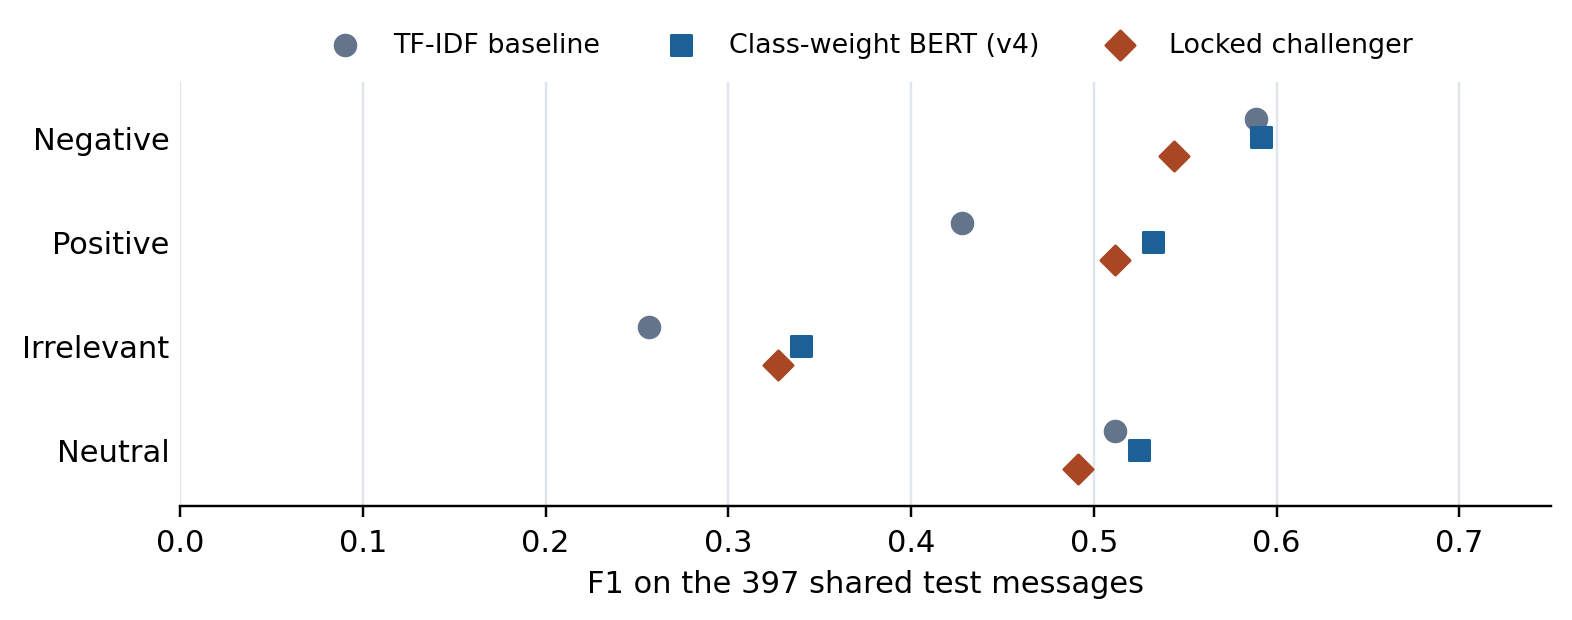
\includegraphics[width=.95\linewidth]{transfer_class_f1.png}\par\smallskip\small\textit{Class F1 for the shared baseline, v4 and the locked challenger.}\end{minipage}\end{center}

\subsection{Performance of the retained model}
The retained v4 configuration scored 0.4971 macro-F1 and 0.5113 accuracy. Against the original baseline its observed macro-F1 gain was 0.0510. The largest class F1 gain was for Positive. For Irrelevant, v4 retrieved 26 of 66 cases compared with 10 for the baseline, with substantially lower precision. For Neutral, v4 retrieved 48 of 105 versus 56 for the baseline. Its higher Neutral precision offset the lower recall in the F1 score.
\begin{center}\begin{minipage}{\linewidth}\centering\small
\begin{tabular}{lrrrrrr}
\toprule
Class & P & R & F1 & $\Delta$P & $\Delta$R & $\Delta$F1 \\
\midrule
Negative & 0.5917 & 0.5917 & 0.5917 & +0.0793 & -0.1000 & +0.0030 \\
Positive & 0.5179 & 0.5472 & 0.5321 & +0.0958 & +0.1132 & +0.1042 \\
Irrelevant & 0.2989 & 0.3939 & 0.3399 & -0.5345 & +0.2424 & +0.0835 \\
Neutral & 0.6154 & 0.4571 & 0.5246 & +0.1242 & -0.0762 & +0.0132 \\
\bottomrule
\end{tabular}
\par\smallskip\textit{Retained class-weight BERT model. Deltas are relative to the original shared baseline.}
\end{minipage}\end{center}

\subsection{Implications for the review queue}
On the shared test messages, v4 routed 87 messages to the Irrelevant category and correctly identified 26 of the 66 actual Irrelevant cases. The challenger routed 99 messages there and identified 27. Automatically suppressing that queue would hide 72 messages carrying one of the other labels. The challenger correctly retained 43 of 105 Neutral messages, compared with 48 for v4. Across all four labels it corrected 5 of v4's mistakes and introduced 18 new ones. A reviewer can use the suggested label to sort messages while preserving the text and its intended entity for inspection.

Two examples from the training-only held-out folds illustrate the label boundary. A photo announcement about Minecraft at Microsoft Inspire (\texttt{train\_449}) was labelled Neutral. Removing the four counts changed its prediction from Positive to Neutral. A comparison of Xbox and PlayStation (\texttt{train\_452}) was also labelled Neutral, but both heads predicted Irrelevant. A product name or opinion-like wording alone does not determine the entity-relative label. These examples were the first corrected and first missed Neutral training rows in source order.


\section{Limitations and reproducibility}
The training and test samples are small. The first study used one seed. The second used three MLP initializations and grouped folds within training, but the same official validation and project test sets were used throughout. The project test set was also inspected in previous experiments, so it cannot be described as a fresh untouched final holdout. A fresh external test set would provide a stronger performance estimate. The second study removed all four original surface counts together. Their individual contributions remain unresolved. For operational use, predictions should support review of the original message and intended entity rather than replace human judgment.

The recorded BERT revision is \texttt{86b5e0934494bd15c9632b12f734a8a67f723594}. The refinement notebook records its split, configuration, per-epoch validation histories, validation comparisons, selected MLP weights, fitted surface scaler, per-row test predictions, metrics, and paired-bootstrap analysis. The standalone notebook and all other members' preprocessing and models must still be combined into the single, well-annotated notebook required by the assignment.

\begin{thebibliography}{9}\raggedright
\bibitem{bert} J. Devlin, M.-W. Chang, K. Lee, and K. Toutanova, ``BERT: Pre-training of deep bidirectional transformers for language understanding,'' in \emph{Proceedings of NAACL-HLT}, 2019, pp. 4171--4186. \url{https://aclanthology.org/N19-1423/}
\bibitem{supcon} P. Khosla et al., ``Supervised contrastive learning,'' in \emph{Advances in Neural Information Processing Systems}, vol. 33, 2020, pp. 18661--18673. \url{https://arxiv.org/abs/2004.11362}
\bibitem{vader} C. J. Hutto and E. Gilbert, \emph{VADER: A parsimonious rule-based model for sentiment analysis of social media text}, ICWSM, 2014. \url{https://github.com/cjhutto/vaderSentiment}
\bibitem{sstbert} TextAttack, \emph{BERT base uncased SST-2}, released checkpoint. \url{https://huggingface.co/textattack/bert-base-uncased-SST-2}
\bibitem{opus} Helsinki-NLP, OPUS-MT English--French and French--English model cards. \url{https://huggingface.co/Helsinki-NLP/opus-mt-en-fr} and \url{https://huggingface.co/Helsinki-NLP/opus-mt-fr-en}
\end{thebibliography}

\end{document}
